\begin{frame}
\frametitle{Our progress}

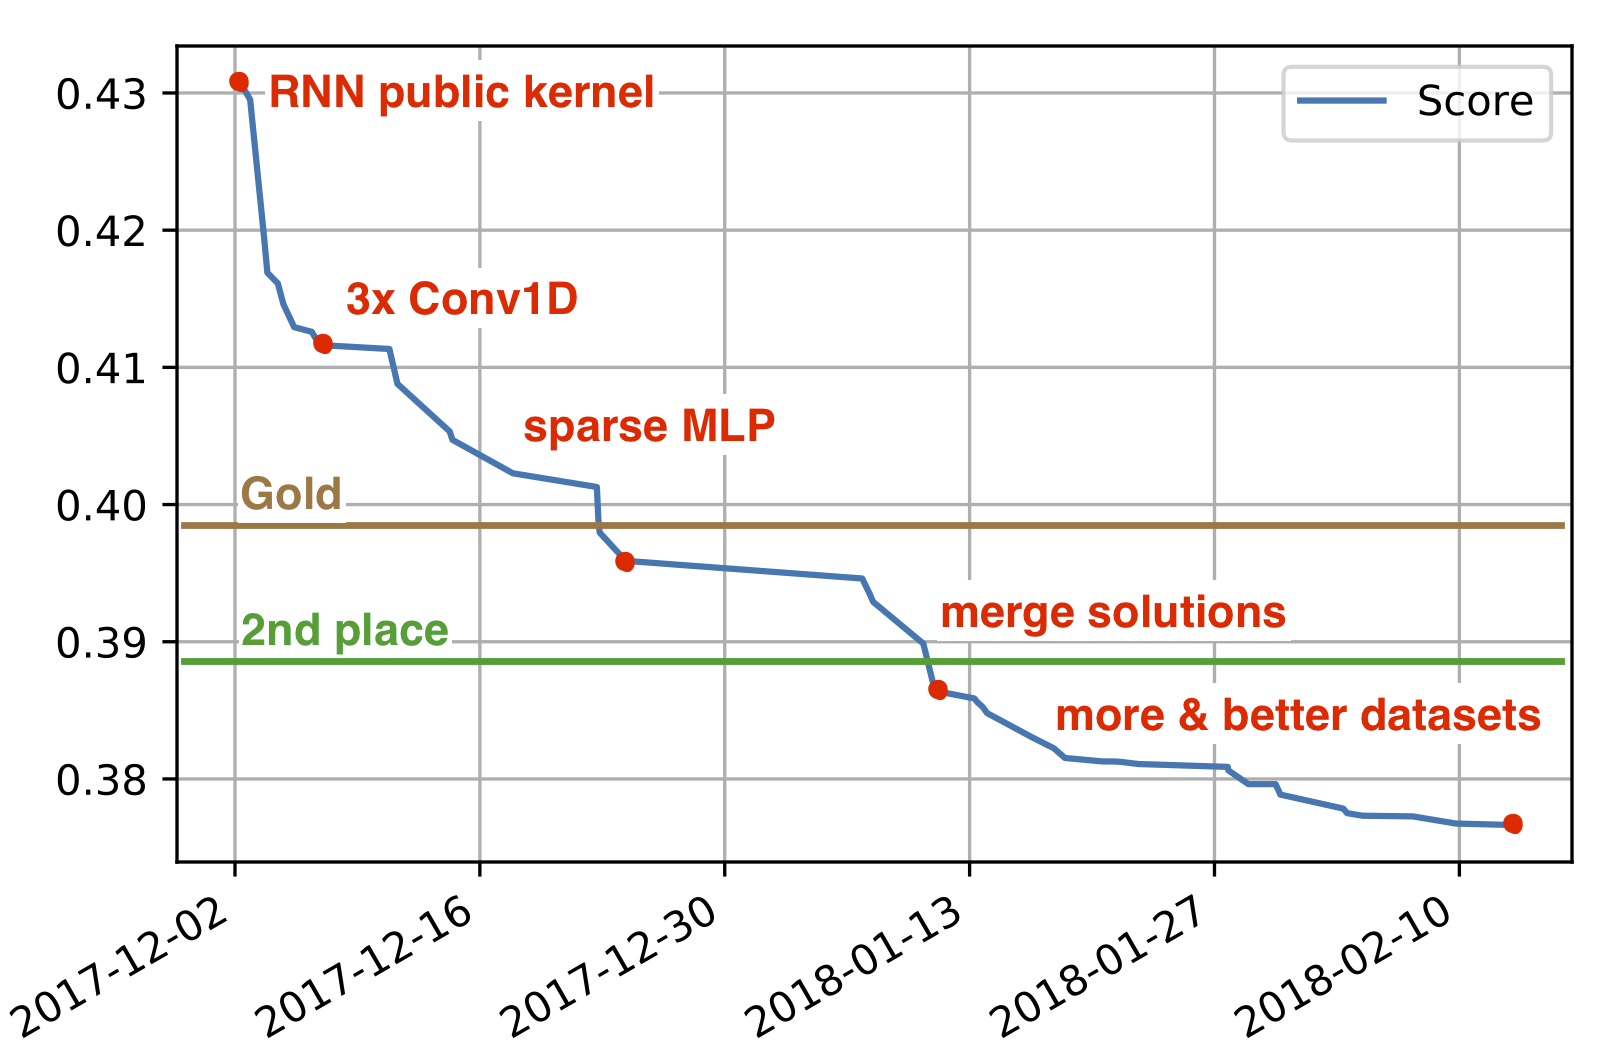
\includegraphics[width=0.85\textwidth]{img/score-chart.png}

\end{frame}

\begin{frame}
\frametitle{To Deep Learn or not to Deep Learn?}

\begin{tabular}{ l | c c }
& Learning & Deep Learning \\
\hline
Architecture & \textbf{MLP} & \textcolor{gray}{LSTM, CNN} \\
Activation & \textcolor{gray}{Tanh} & \textbf{ReLU} \\
Optimization & \textcolor{gray}{SGD} & \textbf{ADAM} \\
Categorical features & \textbf{One-hot encoding} & \textcolor{gray}{Embeddings} \\
\end{tabular}

\end{frame}


\begin{frame}
    \frametitle{Workhorse model: sparse MLP (feedforward neural network)}

    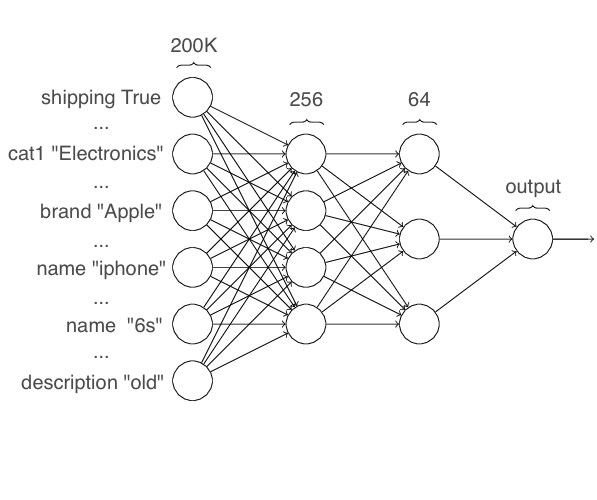
\includegraphics[width=0.85\textwidth]{img/mlp.png}

\end{frame}

\begin{frame}
    \frametitle{Why MLP?}

    \begin{itemize}
        \item Fast to train: can afford hidden size 256 instead of 32--64 for RNN or Conv1D.
        \item Captures interactions between text and categorical features.
        \item Huge variance gives a strong ensemble with a single model type.
    \end{itemize}

\end{frame}


\begin{frame}
    \frametitle{Training}

    Adam, double batch size after each epoch, overfit

    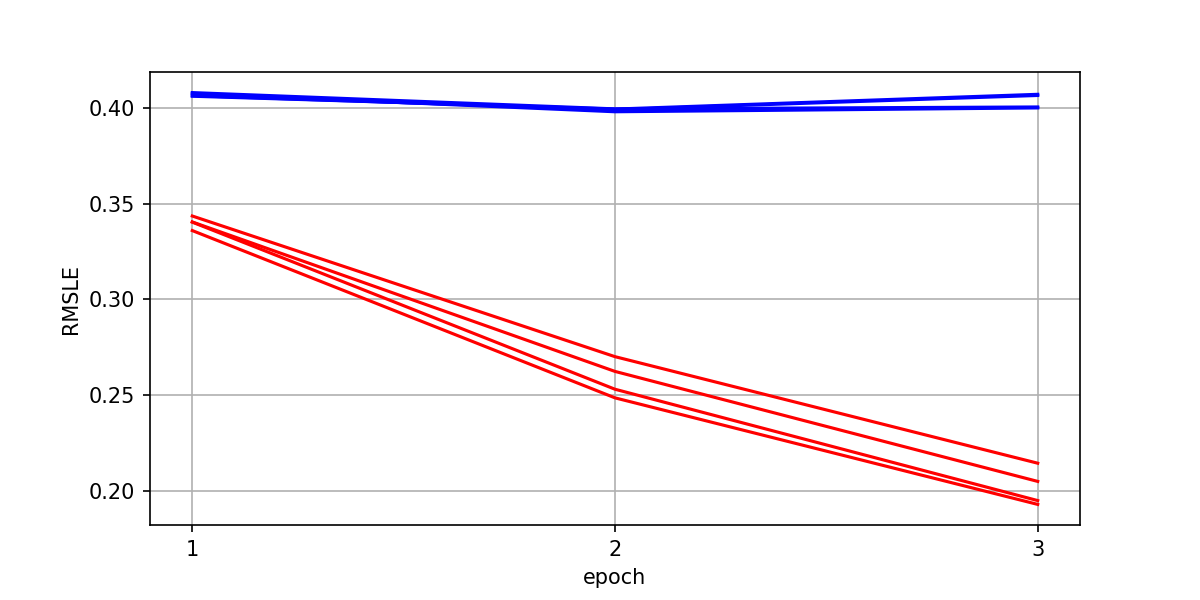
\includegraphics[width=0.85\textwidth]{img/learning_curve_1.png}

\end{frame}

\begin{frame}
    \frametitle{Training}

    Adam, double batch size after each epoch, overfit, profit!

    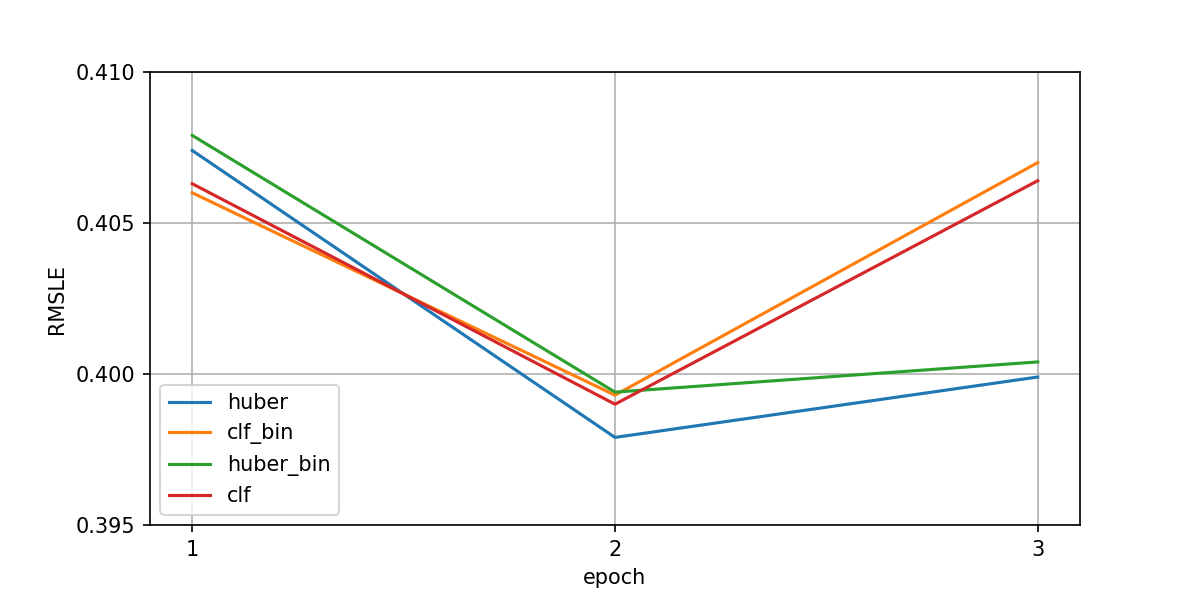
\includegraphics[width=0.85\textwidth]{img/learning_curve_2.png}

\end{frame}


\begin{frame}
    \frametitle{Tricks}

    \begin{itemize}
        \item Huber loss
        \item Regression via. classification
        \item Cheap feature binarization
    \end{itemize}

\end{frame}

\begin{frame}
    \frametitle{Huber Loss}

    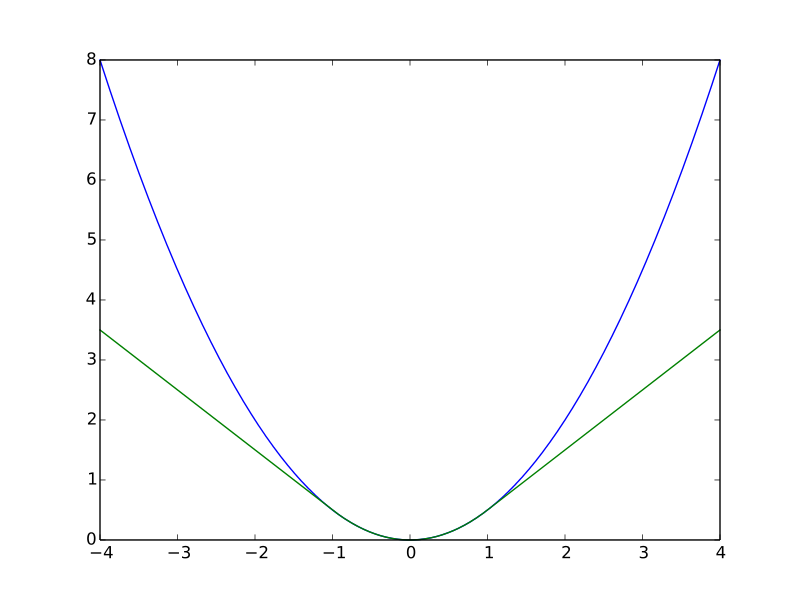
\includegraphics[width=0.75\textwidth]{img/huber.png}

\end{frame}

\begin{frame}
    \frametitle{Regression via Classification}

    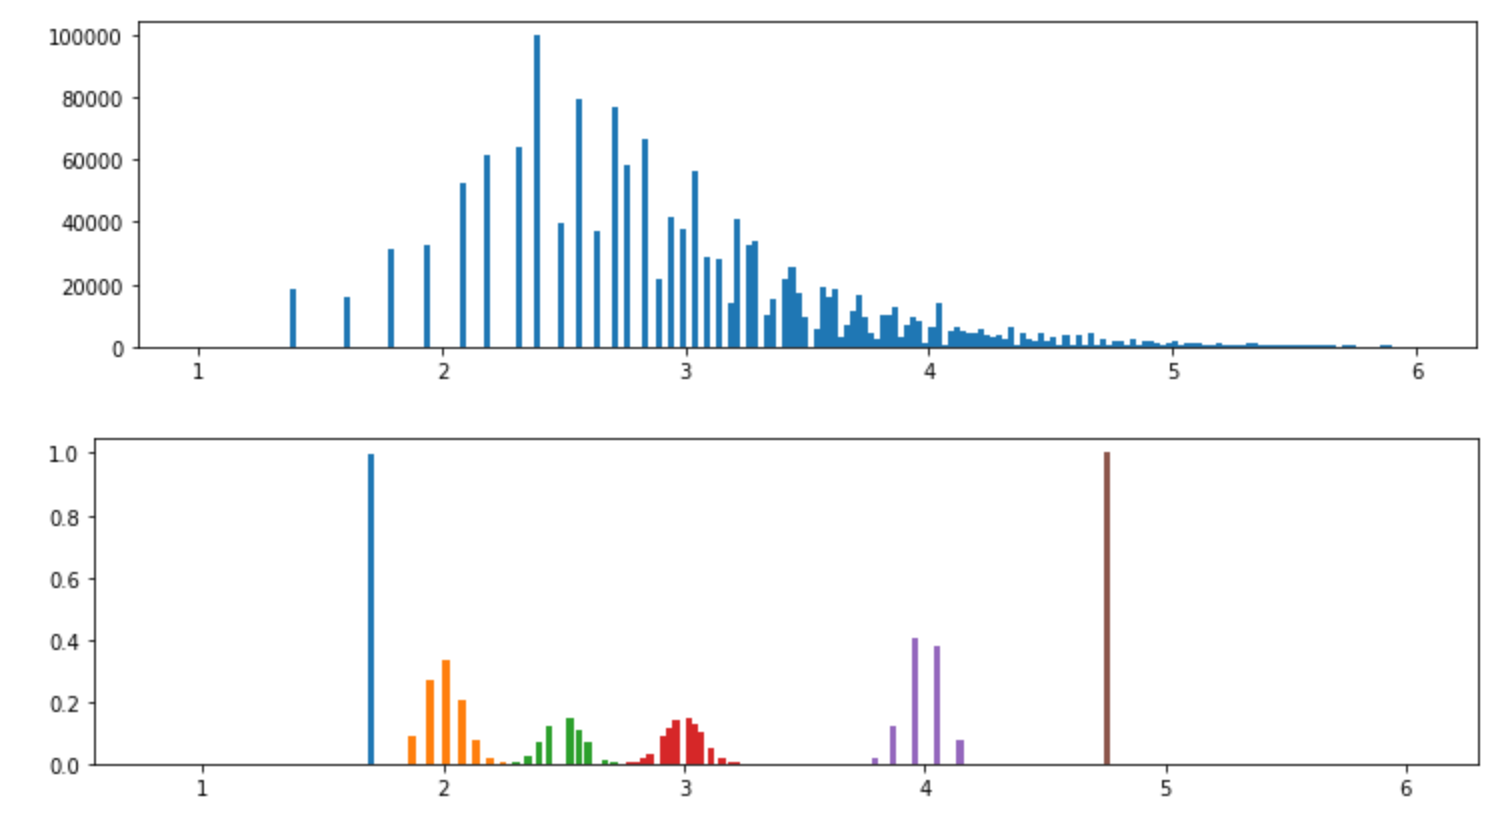
\includegraphics[width=0.95\textwidth]{img/regression_clf.png}

\end{frame}

\begin{frame}
    \frametitle{Cheap feature binarization}

    TF-IDF features $\Rightarrow$ Binary features

    \hspace{3cm}

    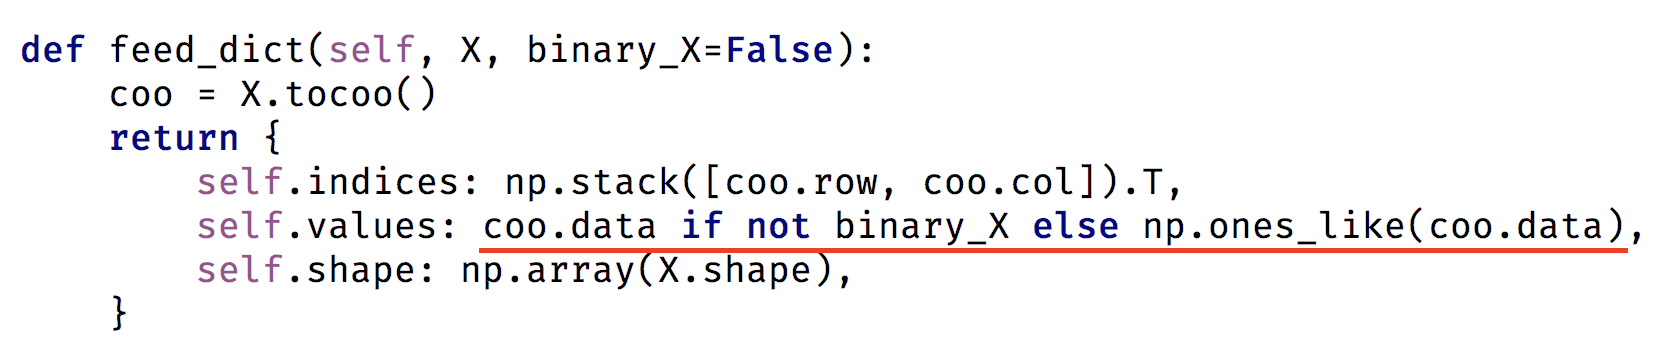
\includegraphics[width=1.0\textwidth]{img/binarization.png}

\end{frame}


\begin{frame}
    \frametitle{Sparse MLP Implementation}

    \begin{itemize}
        \item TensorFlow: \texttt{tf.sparse\_tensor\_dense\_matmul}
        \item MXNet: \texttt{RowSparseNDArray}, sparse updates!
        % https://mxnet.incubator.apache.org/api/python/ndarray/sparse.html
        \item Keras: \texttt{keras.Input(sparse=True)}
        \item Any framework: via embedding
    \end{itemize}

\end{frame}

\begin{frame}
    \frametitle{Optimization: One Model per Core}

    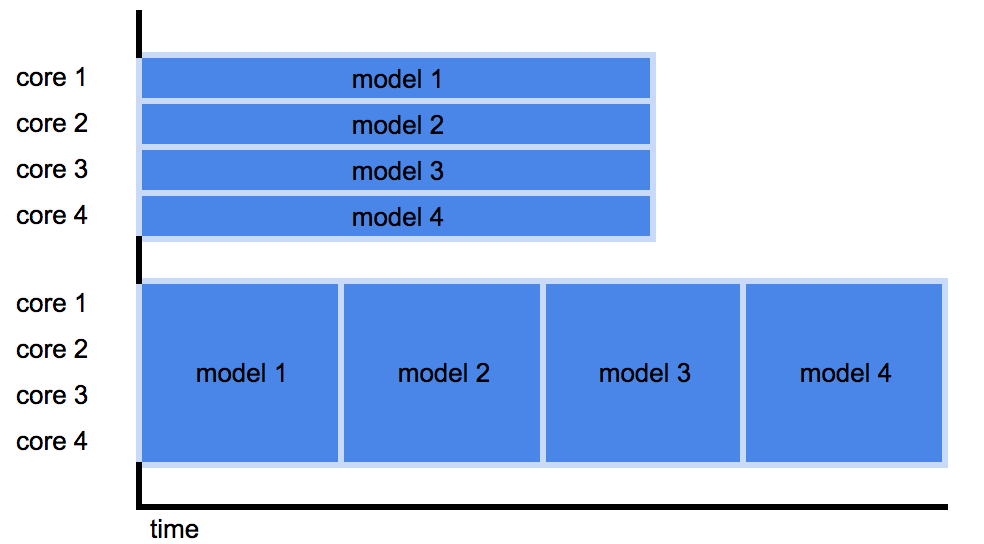
\includegraphics[width=0.85\textwidth]{img/model_per_core.png}

\end{frame}

\begin{frame}
    \frametitle{Optimization: Memory}

    \begin{itemize}
        \item TensorFlow: threading, \texttt{use\_per\_session\_threads}
        \item MXNet: multiprocessing, memory efficient data loader
    \end{itemize}

\end{frame}

\begin{frame}
\frametitle{Ensembling via Lasso}
    5\% local validation, 1\% on Kaggle.
    Very good LB correlation.

    \hspace{2cm}

    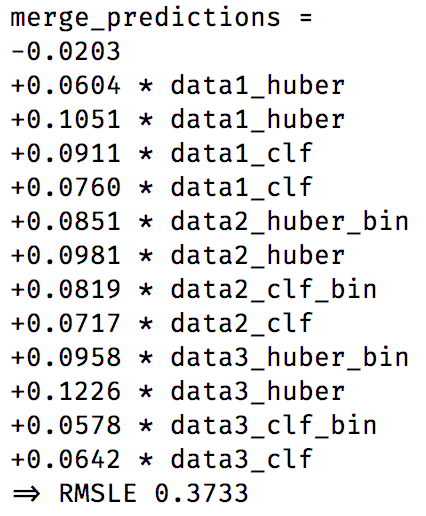
\includegraphics[width=5cm]{img/lasso.png}

\end{frame}

\begin{frame}
    \frametitle{Didn't Work}

    \begin{itemize}
        \item Grid Search
        \item Skip Connections
        \item Mixture of Experts
        \item Factorization Machines
        \item Fitting residuals
    \end{itemize}

\end{frame}
